%%%%%%%%%%%%%%
% To compile the latex source you the following packages
\documentclass[11pt,swedish,a4paper]{article}
\usepackage{color}
\usepackage{listings}
\usepackage{graphicx}
\usepackage{url}
\usepackage[T1]{fontenc}
\usepackage[swedish]{babel}
\usepackage[utf8]{inputenc}
\usepackage[ddmmyyyy]{datetime} 
\renewcommand{\dateseparator}{-}

\definecolor{bbb}{rgb}{.9,.9,.9}
\lstset{stepnumber=2, basicstyle=\small \ttfamily, language=matlab,
  frame=single, framerule=0.pt}

\usepackage[colorlinks=true, pdfstartview=FitV, linkcolor=blue,
citecolor=blue, urlcolor=blue]{hyperref}

\newcommand\kms{$\mathrm{km} \, \mathrm{s}^{-1}$}
\newcommand\kmsmath{\mathrm{km} \, \mathrm{s}^{-1}}



%%%%%%%%%%%%%%%%%%%%%%%%%%%%
%%%%%% Page dimensions %%%%%
%%%%%%  DO NOT CHANGE  %%%%%
%%%%%%%%%%%%%%%%%%%%%%%%%%%%

%\textheight=247mm
\textwidth=163mm
\topmargin=-7mm
\oddsidemargin=-10mm
\evensidemargin=-10mm
%\parindent 10pt

\setlength{\textwidth}{16.3cm}
\setlength{\oddsidemargin}{0cm}
\setlength{\evensidemargin}{0cm}
\addtolength{\textheight}{20mm}
\addtolength{\voffset}{-5mm}
\usepackage{sectsty}
\usepackage[small,bf,hang]{caption}

\allsectionsfont{\sffamily}
\chapterfont{\sffamily}
\chaptertitlefont{\sffamily}


%%%%%%%%%%%%%%%%%%%%%%%%%%%%%
%%%%% Start of document %%%%% 
%%%%%%%%%%%%%%%%%%%%%%%%%%%%%

\begin{document}
\pagestyle{plain}
\pagenumbering{arabic}
\title{\textsf{Att analysera data från SALSA med \textsc{SalsaJ}}}
\author{\textsf{Eskil Varenius}}
\yyyymmdddate
\date{\textsf{Uppdaterad: \today \, \currenttime}}
 

\maketitle

\section*{Sammanfattning}
Detta dokument beskriver hur man analyserar FITS-filer som skapas med 
radioteleskopet SALSA Onsala genom att använda mjukvaran \textsc{SalsaJ}. 
Vi beskriver steg för steg hur du öppnar FITS-filer, förbättrar spektrum
genom att ta bort artefakter från mottagaren (baslinjesubtraktion), och
anpassar Gaussiska intensitetsfördelningar för att mäta hastigheter
och intensiteter för observerade komponenter (toppar).

\tableofcontents

\section{Introduktion}
\label{sec:introduction}

Radioteleskopet SALSA Onsala är en 2.3\,m 
i diameter stor antenn som finns på Onsala Rymdobservatorium utanför
Göteborg. Teleskopet är framtaget för att detektera den svaga strålning
som kommer från vätgas i vår galax Vintergatan. Vätgasen skickar ut 
strålning med våglängd på 21 cm (eller en frekens på 1420.4 MHz). Denna
signal kan detekteras med hjälp av mikrovågsmottagaren som är ansluten
till radioteleskopet. Efter att du gjort observationer med SALSA så kanske
du vill analysera dina data vidare för att få bättre mätvärden än de du
vår direkt i kontrollprogrammet. Via hemsidan så kan du ladda ner dina 
data i FITS-format. Det finns två vanliga sätt att öppna dessa FITS-filer
från SALSA:

\begin{itemize}
\item \textbf{SalsaJ} utvecklades inom projektet EU-HOU. SalsaJ
	kan användas för atta analysera spektral data från SALSA-teleskopet,
	men kan också användas för att titta på annan data, t.ex. astronomiska
	bilder. Den stora fördelen med SalsaJ är att det är enkelt
	att använda och inte kräver några kunskaper om programmering. 
	En nackdel kan vara att det är tidskrävande att analysera många spektra.
\item \textbf{SalsaSpectrum} är ett annat sätt att analysera SALSA-data. 
	Det är ett analyspaket uvecklat i den populära matematiska programvaran
   \textsc{\textsc{Matlab}}. Paketet är skrivet av Daniel Dahlin och 
   skräddarsytt för SALSA-data. Den stora fördelen med SalsaSpectrum är
   att många spektra kan analyseras snabbt. En nackdel kan vara att
   SalsaSpectrum kräver att användaren har en installation av Matlab, vilket
   inte är gratis. Observera att observatoriet inte kan tillhandahålla Matlab,
   men många universitet har gratis tillgång till Matlab för sina studenter.
\end{itemize}
Både SalsaJ och SalsaSpectrum kan laddas ner från hemsidan
{\url{http://vale.oso.chalmers.se/salsa}}. 

\section{Analys av SALSA data med SalsaJ}
\label{sec:salsaj}
I detta avsnitt så beskriver vi steg för steg hur du kan analysera de FITS
filer som skapas av SALSA-teleskopen med hjälp av programmet SalsaJ. Vi
öppnar FITS-filen, ändrar till att visa hastighet, och inspekterar datan
genom att använda muspekaren. Vidare analys, som att ta bort atrefakter
från mottagaren (baslinjesubtraktion), och att anpassa Gaussiska profiler
till topparna, beskrivs i avsnitt. \ref{sect:adv}.
\textbf{VIKTIGT:} SalsaJ kan bara användas för att läsa spektra som skapats 
med SALSA efter 2015-06-23.

\subsection{Starta SalsaJ}
När du laddat hem filen SalsaJ2.jar från hemsidan, öppna den genom att
dubbelklicka. Om detta inte fungerar, prova att högerklicka på filen och välj
\emph{Öppna med} och välj \emph{Java}. När programmet öppnas så bör du se ett
fönster som ser ut ungefär som Fig. \ref{fig:salsajstart}.
\begin{figure}[h!]
  \centering
  \scalebox{0.55}{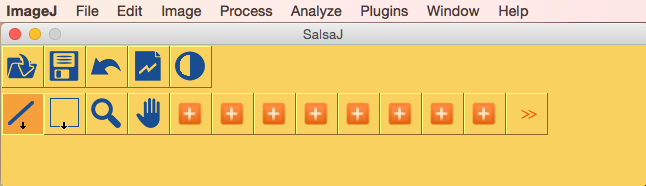
\includegraphics{../figures/start}}
  \caption{Startfönstret för programmet SalsaJ.}
  \label{fig:salsajstart}
\end{figure}

\subsection{Öppna ett spektrum}
För att öppna ett spektrum, d.v.s. en FITS-fil, klicka på menyn \emph{File} 
och sedan på \emph{Radio spectrum}. Leta upp filen som du vill öppna
och klicka på OK. 
Du bör nu se ett spektrum på skärmen, på samma sätt som i Fig. 
\ref{fig:opened}.
\begin{figure}[h!]
  \centering
  \scalebox{0.55}{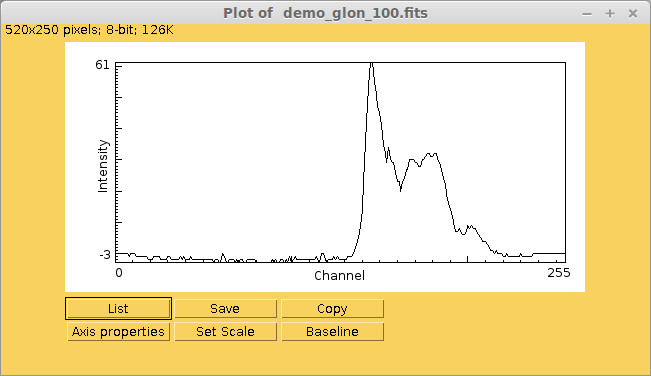
\includegraphics{../figures/spectrumopened}}
  \caption{Ett spektrum har öppnats och 
	  visas som standard med kanalnummer på den horisontella axeln. Vi vill
	  ändra detta till hastighet. 
  }
  \label{fig:opened}
\end{figure}
Obs: Om du använder Mac OS X och inte ser valet \emph{Radio spectrum} 
i menyn \emph{File}, var säker på att du visar menyn för SalsaJ. Du kan 
ta fram menyn för SalsaJ genom att klicka på SalsaJ-fönstret.

\subsection{Hastighet istället för kanal}
Som standard visar SalsaJ ditt spektrum som intensitet vs kanalnummer. I vårt
fall är det mycket mer användbart att byta enhet på den horisontella axeln till
hastighet. Detta kan göras genom att klicka på knappen \emph{Set scale}, 
och sedan välja \emph{Velocity}, och därefter klicka OK. 
Nu bör den horisontella axeln visas i km/s, som i Fig.
\ref{fig:velocity}. Observera att du kan inspektera de uppmätta värdena
genom att flytta pekaren över grafen: intensitet och hastighet visas i 
nedre delen av fönstret. Om du bara är intresserad av ungefärliga värden
av hastitheterna, så kan du skriva ner värdena du hittar genom inspektion
på detta sätt, och sedan vara färdig med detta spektrum. Men, om du vill få
ut bästa möjliga resultat så kan det vara värt att prova baslinjesubtraktion
och Gaussis anpassning som beskrivs i avsnitt 
\ref{sect:adv} nedan.
\begin{figure}[h!]
  \centering
  \scalebox{0.55}{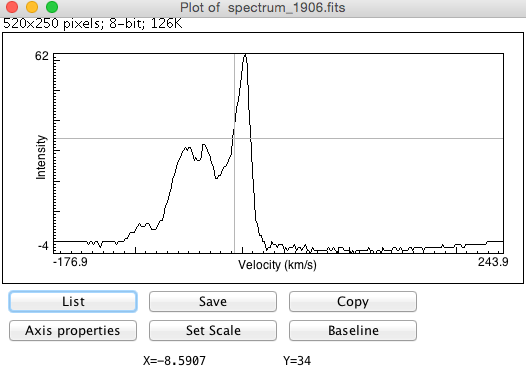
\includegraphics{../figures/spectrumvel}}
  \caption{Detta spektrum visas nu med hastighet på den horisontella
	  axeln. Du kan nu inspektera spektrumet genom att hovra med muspekaren
	  över topparna. Värdet under pekaren visas i nedre delen av fönstret. 
  }
  \label{fig:velocity}
\end{figure}

\section{Avancerad analys}
\label{sect:adv}
För bästa möjliga resultat så kanske du behöver göra en så kallad
baslinjesubtraktion och även gaussisk anpassning av topparna. Detta kan vara
tidskrävande om du har många spektra och överväg att använda Matlab-programmet
SalsaSpectrum om du har tillgång till Matlab.

\subsection{Baslinjesubtraktion}
Spektrat som visas i Fig. \ref{fig:velocity} är ganska bra redan från start, men om 
vi tittar noga så kan vi se att nollnivån inte är platt. Istället så är den böjd
p.g.a. störningar från mottagaren som inte togs bort under observationen. 
För bästa möjliga resultat så måste vi ta bort dessa störningar. Detta borttagande
kallas \emph{baslinjesubtraktion}. Börja genom att klicka på knappen \emph{Baseline} 
i SalsaJ-fönstret. Genom att titta snabbt på grafen med muspekaren ser vi att vi inte
har några toppar mellan [-170 till -130] eller [50 till 240] km/s. 
Vi skriver in dessa gränser för de två linjefria områdena och väljer ett polynom av 
ordning 2, se Fig. \ref{fig:baseline}.

\begin{figure}[h!]
  \centering
  \scalebox{0.55}{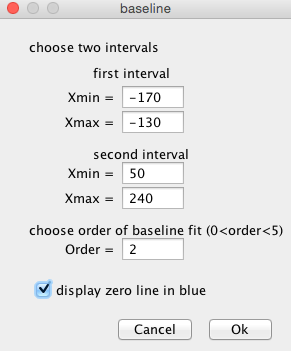
\includegraphics{../figures/baseline}}
  \caption{Inställningar för baslinjesubtraktion. Vi har definierat två regioner
	  av vårt spektrum som är fria från toppar från vätgas, och valt ett ordning på 
	  det polynom som vi vill anpassa (vanligen 2 eller 3). 
  }
  \label{fig:baseline}
\end{figure}

Efter att du trycker på OK så kommer en baslinje att anpassas och visas på skärmen,
se Fig. 
\ref{fig:baselinefit}.
\begin{figure}[h!]
  \centering
  \scalebox{0.55}{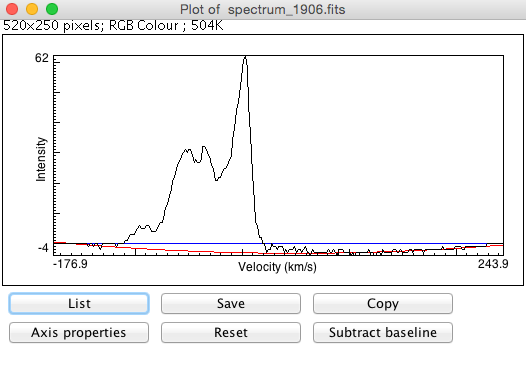
\includegraphics{../figures/baselinefitted}}
  \caption{En baslinje har anpassats baserat på inställningarna i 
	  Fig.  \ref{fig:baseline}. Den anpassade baslinjen visas i rött
	  och noll-nivån i blått.
  }
  \label{fig:baselinefit}
\end{figure}
Om du är nöjd med din anpassning, klicka \emph{Subtract baseline}. Om din anpassning
ser dålig ut, klicka \emph{reset} och gör om subtraktionen med andra inställningar 
tills du får en bra anpassning till de delar av spektrat som är fria från toppar.
Efter att du subtraherat baslinjen så bör de linjefria delarna vara platta, som i Fig. 
\ref{fig:baselinesubtracted}.
\begin{figure}[h!]
  \centering
  \scalebox{0.55}{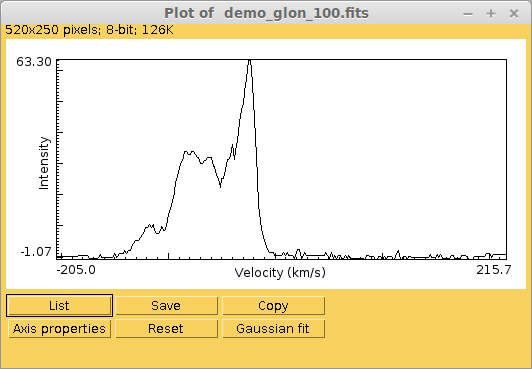
\includegraphics{../figures/baselinesubtracted}}
  \caption{Baslinjen som anpassats i Fig. \ref{fig:baselinesubtracted} har tagits bort
	  och de linjefria områdena är nu platta (bortsett från bruset) och nära noll. Vi
	  är nu redo att mäta intensiteter och hastigheter.
	  }
  \label{fig:baselinesubtracted}
\end{figure}

\subsection{Mätning av hastigheter: att anpassa Gaussiska profiler}
På grund av brus så kan det vara svårt att mäta exakt var centrum av toppen är
bara med hjälp av muspekaren. Ett bra sätt är istället att anpassa en Gaussisk
profil till toppen.  Detta kan göras genom att klicka på knappen \emph{Gaussian
fit} i SalsaJ.  För anpassningen så måste vi först notera ungefärliga värden
för de toppar vi vill anpassa. Här ser vi att vi har fyra toppar ungefär vid
hastigheterna -90, -52, -35, och 0 km/s. Vi vill alltså anpassa fyra toppar,
men SalsaJ kan bara anpassa en åt gången (SalsaSpectrum i Matlab kan anpassa
flera samtidigt) Låt oss börja med den starkaste toppen kring 0.

Efter att vi klickar på knappen \emph{Gaussian fit} så behöver vi ange ett interval 
med data som skall användas för anpassningen, definierat med Xmin och Xmax. Vanligen så
funkar ett område av 10km/s till höger och vänster om toppen bra, så i detta fall 
-10 till +10 km/s. Därefter måste vi ge startvillkor för anpassningen. Detta måste inte vara
perfekt, men ju närmare desto bättre. Vi gissar på en amplitud på 30 (vilket är långt
under den riktiga amplituden), ett center på 0 (som vi noterade innan) och en bredd på
20km/s. Sen klickar på OK. Den anpassade profilen visas i rött, se Fig. 
\ref{fig:fittedgaussian}. 

Obs: Om din anpassning går fel, t.ex. om du anger ett interval där det inte
finns någon topp, så kan du ta bort den senaste anpassningen genom att välja
\emph{erase the last}. 

Vi fortsätter att på samma sätt anpassa de övriga tre topparna, resultatet kan
ses i Fig.  \ref{fig:allfitted}. Efter anpassning så får du en lista av
anpassade värden, se Fig.  \ref{fig:fitres}. Ur denna lista så kan du läsa av
galaktiska koordinater för spektrat, och de hastigheter och intensiteter som
programmet anpassat för de toppar du valt.  Hastigheterna kan sedan användas
för att göra en rotationskurva eller en karta över Vintergatan på det sätt som
beskrivs i projektbeskrivningen Kartläggning av Vintergatan. 


\begin{figure}[h!]
  \centering
  \scalebox{0.55}{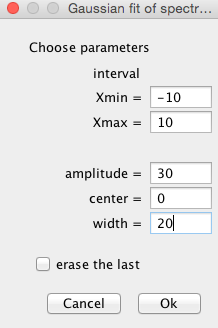
\includegraphics{../figures/fitpars}}
  \caption{Inställningar för att anpassa en gaussisk profil
	  till en av topparna i spektrat. Resultatet kan ses i Fig. 
  \ref{fig:fittedgaussian}.} \label{fig:fitpars}
\end{figure}

\begin{figure}[h!]
  \centering
  \scalebox{0.55}{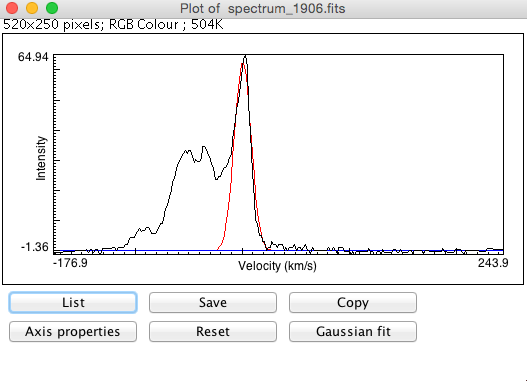
\includegraphics{../figures/fittedgauss}}
  \caption{En gaussisk profil har anpassats till datan
	  utifrån inställningarna i Fig. 
  \ref{fig:fitpars}.} \label{fig:fittedgaussian}
\end{figure}

\begin{figure}[h!]
  \centering
  \scalebox{0.55}{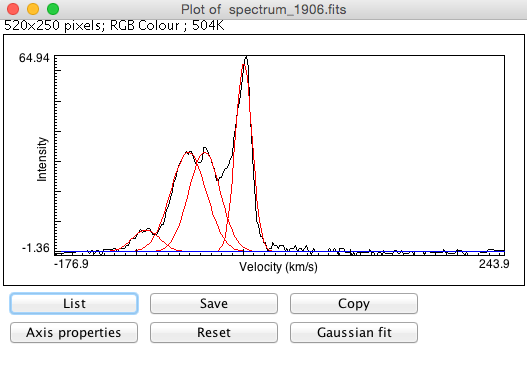
\includegraphics{../figures/allfitted}}
  \caption{Alla fyra toppar har anpassats. Hastigheter och intensiteter
	  kan nu avläsas i \emph{Gaussian fit results}, se Fig. \ref{fig:fitres}.} \label{fig:allfitted}
\end{figure}

\begin{figure}[h!]
  \centering
  \scalebox{0.55}{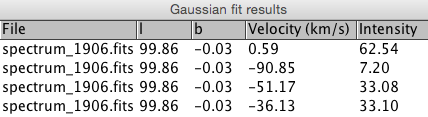
\includegraphics{../figures/fitres}}
  \caption{Alla fyra toppar har anpassats. I detta fönster kan du läsa av de anpassade
	  hastigheterna och intensiteterna. Värdena kan användas för att göra en rotationskurva
	  eller karta för Vintergatan, på det sätt som beskrivs i projektbeskrivningen
	  Kartläggning av Vintergatan. 
  } \label{fig:fitres}
\end{figure}


\end{document}

